\section{自适应更新}
\label{sec:sgdb-adaptive}

动量决定历史读数怎样合成方向。本节研究历史读数的另一种用途：根据过去读数的幅度，决定每个坐标或每个矩阵方向的更新尺度。不同坐标的读数幅度可能相差几个量级，同一个步长对它们不合适。这些方法都写成
\begin{equation}
 \bm{x}^{(t+1)}=\bm{x}^{(t)}-\alpha^{(t)}\bm{D}^{(t)}\hat{\bm g}^{(t)},
 \label{eq:sgdb-adaptive-form}
\end{equation}
或把$\hat{\bm g}^{(t)}$换成动量方向，其中$\bm{D}^{(t)}$是由历史读数算出的缩放。

$\bm{D}^{(t)}$的算法各不相同，但有一个共同的分析障碍：尺度和当前读数通常相关。如果$\bm{D}^{(t)}$在本轮抽样之前已经确定，它可以从条件期望中提到外面；这里不行，$\bm{D}^{(t)}$往往用到了本轮读数。一元的第一步最能说明问题。设累计统计用本轮读数，则第一步的方向是
\[
 \frac{\hat g}{\sqrt{\hat g^2}}=\operatorname{sign}(\hat g).
\]

在贯穿例的$x^{(0)}=2$处，三项读数是$5,4,-3$。缩放后的方向分别是$1,1,-1$，条件均值为
\[
 \frac13\bigl(1+1-1\bigr)=\frac13,
\]
而$f'(2)=2$。这个差别不是一个固定的比例因子：缩放后的条件均值由读数的分布决定，与$f'(2)$的大小没有固定关系。

所以下面每个方法都要写清统计量的更新次序，并分开说明保证所依赖的假设。全节沿用贯穿例的三轮读取，步长记作$\alpha$，稳定项$\epsilon>0$在手算中忽略。所有除法、平方根和乘方都逐坐标进行，$\odot$表示逐元素乘法。

\subsection{AdaGrad}
\label{sec:sgdb-adagrad}

\paragraph{累计平方与稀疏坐标}
设想一个分类问题，特征是某些词是否出现。常见词在几乎每个样本中出现，对应坐标的读数频繁非零；罕见词偶尔才出现。用同一个步长，罕见词的坐标几乎没有机会被更新。AdaGrad为每个坐标累计读数的平方，用它的平方根缩放当前读数\scite{duchi2011adagrad}。取$\bm{s}^{(0)}=\bm{0}$，读数之后先更新统计，再用新统计更新参数：
\begin{equation}
 \bm{s}^{(t+1)}=\bm{s}^{(t)}+\hat{\bm g}^{(t)}\odot\hat{\bm g}^{(t)},\qquad
 \bm{x}^{(t+1)}=\bm{x}^{(t)}-\alpha\frac{\hat{\bm g}^{(t)}}{\sqrt{\bm{s}^{(t+1)}}+\epsilon}.
 \label{eq:sgdb-adagrad}
\end{equation}

这里$\bm{s}$是累计统计，$\epsilon$只防止分母为零。第$j$个坐标的有效系数是$\alpha/(\sqrt{s_j^{(t+1)}}+\epsilon)$。读数频繁非零的坐标累计得快，系数缩小得快；稀疏坐标累计得慢，系数保持较大。

\paragraph{两个坐标的短序列}
下面用一个短序列计算有效系数。取$\alpha=1$，忽略$\epsilon$。坐标$1$每轮读数都是$1$，坐标$2$只在$t=0$和$t=3$读数为$1$，其余轮读数为零，不发生位移。表~\ref{tab:sgdb-adagrad-steps}列出每轮作用在非零读数上的系数。

\begin{BookInlineTable}
  \centering
  \caption{有效系数$\alpha/\sqrt{s_j^{(t+1)}}$的比较，$\alpha=1$，忽略稳定项。坐标$2$只在$t=0,3$读数为$1$，其余轮读数为零，记作“—”。RMSProp取$\rho=0.9$。}
  \label{tab:sgdb-adagrad-steps}
  \begin{tabular}{ccccc}
    \toprule
    & \multicolumn{2}{c}{AdaGrad} & \multicolumn{2}{c}{RMSProp}\\
    \cmidrule(lr){2-3}\cmidrule(lr){4-5}
    轮次$t$ & 坐标$1$ & 坐标$2$ & 坐标$1$ & 坐标$2$\\
    \midrule
    $0$ & $1.000$ & $1.000$ & $3.162$ & $3.162$\\
    $1$ & $0.707$ & — & $2.294$ & —\\
    $2$ & $0.577$ & — & $1.921$ & —\\
    $3$ & $0.500$ & $0.707$ & $1.705$ & $2.405$\\
    $4$ & $0.447$ & — & $1.563$ & —\\
    $5$ & $0.408$ & — & $1.461$ & —\\
    \bottomrule
  \end{tabular}
\end{BookInlineTable}

AdaGrad的两列中，坐标$1$的系数按$1/\sqrt{t+1}$持续缩小，到$t=3$是$0.5$；坐标$2$到$t=3$才累计了两次，系数是$0.707$。稀疏的坐标因此保留了较大的步长。

累计统计的问题是不会忘记旧尺度。设某坐标前$10$轮的读数幅度是$10$，之后幅度都是$1$。前$10$轮累计了$1000$，此后每轮只增加$1$，到第$80$轮累计量约为$1070$，系数约为$0.031$。图~\ref{fig:sgdb-adagrad-forget}(b)中的黄线显示了这一点：早期的大读数使有效系数永久偏小，算法可能在远离解时就几乎不再移动。

\begin{BookInlineFigure}
  \centering
  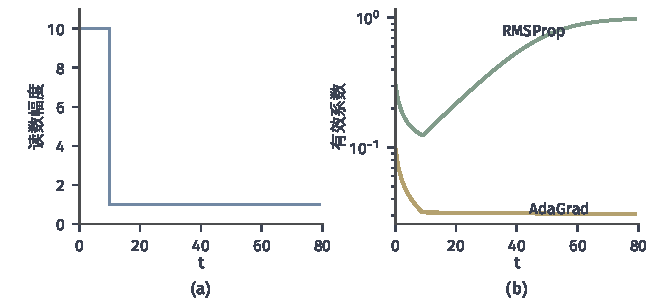
\includegraphics[width=112mm]{figures/05-optimization/05-stochastic-optimization/matplotlib/sgdb-adagrad-forget/figure.pdf}
  \caption{同一读数序列下的有效系数，$\alpha=1$，忽略稳定项。(a)读数幅度：前$10$轮为$10$，之后为$1$。(b)有效系数的对数图。黄线是AdaGrad，累计统计使系数一直偏小；绿线是$\rho=0.9$的RMSProp，大读数被遗忘后系数恢复到接近$1$。}
  \label{fig:sgdb-adagrad-forget}
\end{BookInlineFigure}

\paragraph{保证的范围}
AdaGrad的额外状态是一个$n$维向量，每轮额外计算量$O(n)$。保证按问题类型分别成立，引用时要注明。

\begin{itemize}
 \item 凸在线问题：对手依次给出凸损失，算法在有界可行域上行动，读数有界。评价对象是遗憾，也就是累计损失减去最好的固定决策的累计损失。原始分析给出$O(\sqrt T)$的遗憾，并在读数稀疏时有更好的常数\scite{duchi2011adagrad}。
 \item 随机凸问题：读数条件无偏时，可以由在线遗憾得到平均迭代的期望目标差，量级是$O(1/\sqrt T)$，同样需要有界可行域或相应的有界假设。
 \item 非凸光滑问题：评价对象是平方梯度范数的平均，需要读数有界或其他尾部条件，分母里的当前读数一般要特别处理。这类结果依赖具体的算法形式和假设，不能从凸的情形类推。
\end{itemize}

从更新形式本身推不出“比梯度下降快”。逐坐标缩放只有在问题的难点与坐标轴对齐时才有优势，图~\ref{fig:sgdb-adaptive-rotation}会展示这一边界。

\subsection{RMSProp}
\label{sec:sgdb-rmsprop}

\paragraph{用指数移动平均遗忘旧尺度}
AdaGrad难以遗忘，RMSProp把累计和换成\term{指数移动平均}（exponential moving average）\scite{hinton2012rmsprop}。取衰减系数$\rho\in[0,1)$，$\bm{s}^{(0)}=\bm{0}$：
\begin{equation}
 \bm{s}^{(t+1)}=\rho\bm{s}^{(t)}+(1-\rho)\hat{\bm g}^{(t)}\odot\hat{\bm g}^{(t)},\qquad
 \bm{x}^{(t+1)}=\bm{x}^{(t)}-\alpha\frac{\hat{\bm g}^{(t)}}{\sqrt{\bm{s}^{(t+1)}}+\epsilon}.
 \label{eq:sgdb-rmsprop}
\end{equation}

顺序与AdaGrad相同：先读，再用本轮读数更新$\bm{s}$，最后用新统计缩放本轮读数。$\epsilon$放在根号外，有的实现把它放在根号内，两者在分母很小时行为不同，记录实现时要写明。

展开递推，得到
\[
 \bm{s}^{(t+1)}=(1-\rho)\sum_{r=0}^{t}\rho^{t-r}\hat{\bm g}^{(r)}\odot\hat{\bm g}^{(r)}.
\]

$s$轮之前的读数平方的权重是$(1-\rho)\rho^{s}$，大约只记住最近$1/(1-\rho)$轮。$\rho=0.9$时约为$10$轮。

\paragraph{零初始化的早期偏差}
权重之和是$1-\rho^{t+1}$，早期小于$1$。读数恒为$g$时，
\[
 s^{(t+1)}=\bigl(1-\rho^{t+1}\bigr)g^2 ,
\]
早期分母偏小，有效系数偏大。表~\ref{tab:sgdb-adagrad-steps}的RMSProp列中，第一轮的系数是$1/\sqrt{0.1}\approx3.162$，比AdaGrad大得多。

再看图~\ref{fig:sgdb-adagrad-forget}的序列：前$10$轮把分母抬到约$8$，读数变小后，统计量大约以因子$\rho$逐轮衰减。第$30$轮的有效系数已经回到约$0.35$，第$79$轮约为$0.98$。

指数平均让尺度跟上最近的幅度，但它不提供一般的收敛保证。分母可能在大读数过后迅速变小，有效系数随之变大，下一节将看到这在特定问题上可能破坏收敛。

\subsection{Adam}
\label{sec:sgdb-adam}

\paragraph{主要思想}
RMSProp的分子只用当前读数。Adam在分子上也用移动平均，并修正两个平均的零初始化偏差\scite{kingma2015adam}。取$\beta_1,\beta_2\in[0,1)$，一阶统计$\bm{m}$与平方统计$\bm{s}$从零开始，读取本轮读数后依次计算
\begin{equation}
 \begin{aligned}
 \bm{m}^{(t+1)}&=\beta_1\bm{m}^{(t)}+(1-\beta_1)\hat{\bm g}^{(t)},\\
 \bm{s}^{(t+1)}&=\beta_2\bm{s}^{(t)}+(1-\beta_2)\hat{\bm g}^{(t)}\odot\hat{\bm g}^{(t)}.
 \end{aligned}
 \label{eq:sgdb-adam-stats}
\end{equation}

零初始化带来的偏差如何修正？展开$\bm{m}^{(t+1)}$，权重是$(1-\beta_1)\beta_1^{t-r}$，加起来是$1-\beta_1^{t+1}$，不是$1$。把统计量除以权重之和，得到两个修正量：
\begin{equation}
 \hat{\bm m}^{(t+1)}=\frac{\bm{m}^{(t+1)}}{1-\beta_1^{t+1}},\qquad
 \hat{\bm s}^{(t+1)}=\frac{\bm{s}^{(t+1)}}{1-\beta_2^{t+1}}.
 \label{eq:sgdb-adam-correction}
\end{equation}
读数恒为常数$\bm{g}$时，修正后$\hat{\bm m}^{(t+1)}=\bm{g}$，$\hat{\bm s}^{(t+1)}=\bm{g}\odot\bm{g}$，每一轮都恰好是常数读数的值。

参数更新使用修正后的量：
\begin{equation}
 \bm{x}^{(t+1)}=\bm{x}^{(t)}-\alpha\frac{\hat{\bm m}^{(t+1)}}{\sqrt{\hat{\bm s}^{(t+1)}}+\epsilon}.
 \label{eq:sgdb-adam-update}
\end{equation}

\begin{BookInlineFigure}
  \centering
  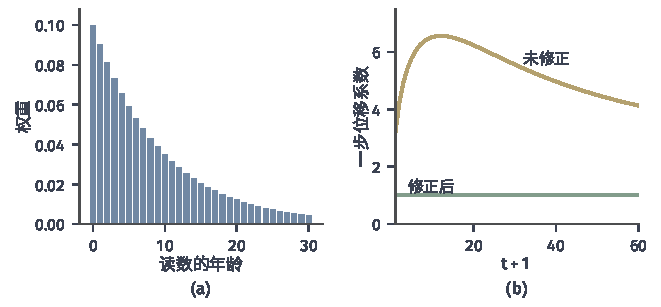
\includegraphics[width=112mm]{figures/05-optimization/05-stochastic-optimization/matplotlib/sgdb-adam-correction/figure.pdf}
  \caption{Adam的零初始化修正，$\beta_1=0.9$，$\beta_2=0.999$，读数恒为$1$，忽略稳定项。(a)$\bm{m}$的权重$(1-\beta_1)\beta_1^{s}$，$s$是读数的年龄。(b)一步位移的系数：黄线是未修正的$m/\sqrt{s}$，第一步约$3.16$，之后更大；绿线是修正后的$\hat m/\sqrt{\hat s}$，恒为$1$。}
  \label{fig:sgdb-adam-correction}
\end{BookInlineFigure}

图~\ref{fig:sgdb-adam-correction}(b)说明了修正的必要。$\beta_2$很接近$1$时，$\bm{s}$起步慢，未修正的$m/\sqrt{s}$在前几十轮都明显偏大，第$10$轮约为$6.5$。修正后系数恒为$1$。

\needspace{6\baselineskip}
\paragraph{变量}
\begin{itemize}
 \item $\bm{x}^{(t)}\in\mathbb{R}^n$：参数。
 \item $\bm{m}^{(t)},\bm{s}^{(t)}\in\mathbb{R}^n$：读数的一阶统计与平方统计。
 \item $t$：计时器，决定修正因子。
 \item $\alpha>0$，$\beta_1,\beta_2\in[0,1)$，$\epsilon>0$：步长、两个衰减系数、稳定项。
\end{itemize}

\paragraph{初始化}
令$\bm{m}^{(0)}=\bm{s}^{(0)}=\bm{0}$，$t=0$。例中是贯穿例的三项目标，取$\alpha=0.1$，$\beta_1=0.9$，$\beta_2=0.999$，读取顺序为第$3,1,2$项，手算时忽略$\epsilon$，起点和统计是
\[
 x^{(0)}=2,\qquad m^{(0)}=0,\qquad s^{(0)}=0.
\]

\needspace{6\baselineskip}
\paragraph{每轮更新}
在第$t$轮依次执行：
\begin{enumerate}
 \item \textbf{读取。}在当前点读取$\hat{\bm g}^{(t)}$。例中第一轮
 \[
  \hat g^{(0)}=f_3'(2)=-3.
 \]
 \item \textbf{更新统计。}按式~\eqref{eq:sgdb-adam-stats}计算$\bm{m}^{(t+1)}$和$\bm{s}^{(t+1)}$。例中第一轮
 \[
  m^{(1)}=0.1\cdot(-3)=-0.3,\qquad s^{(1)}=0.001\cdot9=0.009.
 \]
 \item \textbf{修正。}按式~\eqref{eq:sgdb-adam-correction}计算修正量。例中第一轮
 \[
  \hat m^{(1)}=\frac{-0.3}{0.1}=-3,\qquad \hat s^{(1)}=\frac{0.009}{0.001}=9.
 \]
 \item \textbf{更新参数。}按式~\eqref{eq:sgdb-adam-update}更新，然后$t\leftarrow t+1$。例中第一轮
 \[
  x^{(1)}=2-0.1\cdot\frac{-3}{3}=2.1.
 \]

 第二轮抽到第$1$项，读数和统计是
 \[
  \hat g^{(1)}=5.1,\qquad m^{(2)}=0.24,\qquad s^{(2)}=0.035001.
 \]
 两个修正分母是$1-0.81=0.19$和$1-0.998001=0.001999$，于是
 \[
  \hat m^{(2)}\approx1.2632,\qquad \hat s^{(2)}\approx17.509,\qquad \sqrt{\hat s^{(2)}}\approx4.184,
 \]
 参数更新为
 \[
  x^{(2)}=2.1-0.1\cdot\frac{1.2632}{4.184}\approx2.0698.
 \]

 第三轮抽到第$2$项，读数和统计是
 \[
  \hat g^{(2)}\approx4.1396,\qquad m^{(3)}\approx0.6300,\qquad s^{(3)}\approx0.052102.
 \]
 修正后
 \[
  \hat m^{(3)}\approx2.3246,\qquad \hat s^{(3)}\approx17.385,\qquad \sqrt{\hat s^{(3)}}\approx4.170,
 \]
 参数更新为
 \[
  x^{(3)}\approx2.0698-0.0558=2.0141.
 \]
\end{enumerate}

按预定轮数结束，例中$T=3$，最终得到$x^{(3)}\approx2.0141$。

\paragraph{修正偏差与优化方向的偏差}
修正因子只消除零初始化造成的权重不足，它不说明优化方向没有偏差。在上面的例子中，第二轮开始前$x^{(1)}=2.1$，$f'(2.1)=2.2$。固定历史后，$m^{(2)}$的条件均值是$0.9\cdot(-0.3)+0.1\cdot2.2=-0.05$，修正后的分子的条件均值约为
\[
 \frac{-0.05}{0.19}\approx-0.263 .
\]
它的符号甚至与$f'(2.1)$相反，原因是分子包含了上一轮的反向读数。分母还依赖本轮读数，所以式~\eqref{eq:sgdb-adam-update}的方向既不是当前梯度的无偏估计，也不是确定矩阵乘以当前梯度。

\paragraph{状态与保证}
Adam的状态包括$\bm{x}$、$\bm{m}$、$\bm{s}$和计时$t$。恢复运行时四项都要恢复：只恢复参数会丢失方向记忆；$t$错了，修正因子就错了。

Adam的原始论文给出了凸在线问题的分析，后来发现证明中存在问题，并有反例说明算法在一些凸问题上不收敛，下一小节说明这一点。引用Adam的保证时，必须对应具体的问题假设和参数设置，不能把一个具体分析中的结论当成算法的一般性质。

\paragraph{逐坐标缩放的边界}
图~\ref{fig:sgdb-adaptive-rotation}用精确梯度比较三种方法。目标是$f=(x_1^2+9x_2^2)/2$，起点$(9,1)$。主轴与坐标轴对齐时，AdaGrad第一步是$\alpha(1,1)$，随后逐坐标的尺度抵消了两个方向的曲率差异，到第$60$轮目标值约为$10^{-13}$。把目标和起点一起旋转$45^\circ$，陡峭方向不再对应一个坐标，AdaGrad到第$60$轮目标值约为$10^{-8}$，下降明显变慢。梯度下降对旋转不变，实线和虚线重合。

\begin{BookInlineFigure}
  \centering
  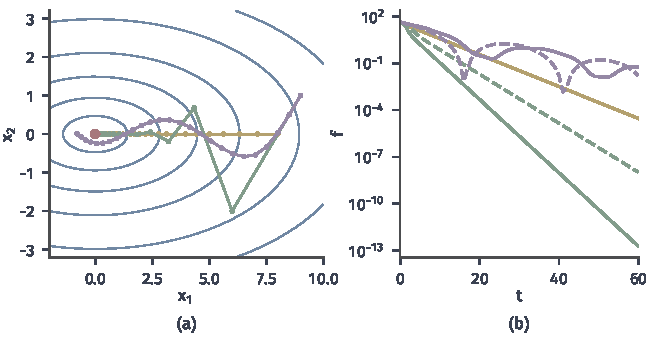
\includegraphics[width=112mm]{figures/05-optimization/05-stochastic-optimization/matplotlib/sgdb-adaptive-rotation/figure.pdf}
  \caption{逐坐标缩放与坐标系。目标$f=(x_1^2+9x_2^2)/2$，起点$(9,1)$，精确梯度。黄线是$\alpha=1/9$的梯度下降，绿线是$\alpha=3$的AdaGrad，紫线是$\alpha=0.5$的Adam（$\beta_1=0.9$，$\beta_2=0.999$）。(a)前$25$步的路径。(b)目标值：实线为原问题，虚线为把目标与起点一起旋转$45^\circ$后的同一问题，两条黄线重合。}
  \label{fig:sgdb-adaptive-rotation}
\end{BookInlineFigure}

\subsection{AMSGrad}
\label{sec:sgdb-amsgrad}

\paragraph{分母可能回落}
Adam和RMSProp的分母是指数平均，大读数过后可能迅速变小。分母一变小，有效步长就变大，此时的小读数被放大。这会造成什么后果？下面的构造说明，它足以让算法在一个凸问题上走向错误的方向\scite{reddi2018amsgrad}。

可行集是$[-1,1]$，读数依周期$3$变化，$C>2$：
\[
 \hat g^{(t)}=\begin{cases}C,& t\equiv1\pmod3,\\-1,&\text{其他}.\end{cases}
\]
对应的线性损失为$f_t(x)=\hat g^{(t)}x$，一个周期的总损失是$(C-2)x$，最优解是$x=-1$。取$C=3$，$\beta_1=0$（不用动量），$\beta_2=1/(1+C^2)=0.1$，步长$\alpha^{(t)}=0.1/\sqrt t$，更新后投影回$[-1,1]$。

\paragraph{一个周期内的净位移}
分母的三个值在稳态时循环。$s$按式~\eqref{eq:sgdb-adam-stats}递推，大读数$C$进入时升到约$8.207$，之后依次回落到$1.721$和$1.072$，所以一个周期的三个除数约为
\[
 \sqrt{8.207}\approx2.865,\qquad \sqrt{1.721}\approx1.312,\qquad \sqrt{1.072}\approx1.035.
\]
三步的位移与步长之比分别是$-3/2.865$，$+1/1.312$，$+1/1.035$，合计
\[
 -1.047+0.762+0.966=+0.681>0.
\]
一个周期的净位移是正的，迭代被推向错误的边界$x=+1$。大读数被大分母压低，小读数被回落的分母放大，方向信息就颠倒了。

\paragraph{算法}
AMSGrad让分母只增不减。分子和分母都不作零初始化修正，把历史最大的平方统计放进分母\scite{reddi2018amsgrad}。取$\bar{\bm s}^{(0)}=\bm{0}$，每轮在式~\eqref{eq:sgdb-adam-stats}之后计算
\begin{equation}
 \bar{\bm s}^{(t+1)}=\max\bigl\{\bar{\bm s}^{(t)},\bm{s}^{(t+1)}\bigr\},\qquad
 \bm{x}^{(t+1)}=\bm{x}^{(t)}-\alpha^{(t)}\frac{\bm{m}^{(t+1)}}{\sqrt{\bar{\bm s}^{(t+1)}}+\epsilon},
 \label{eq:sgdb-amsgrad}
\end{equation}
其中$\max$逐坐标取。

在上面的例子中，$\bar s$稳定在$8.207$，一个周期的位移与步长之比变为
\[
 \frac{-3+1+1}{2.865}\approx-0.349<0,
\]
净位移转为负，迭代走向$x=-1$。图~\ref{fig:sgdb-amsgrad-counter}的实际运行与此一致：Adam趋于$+1$，AMSGrad趋于$-1$。

\begin{BookInlineFigure}
  \centering
  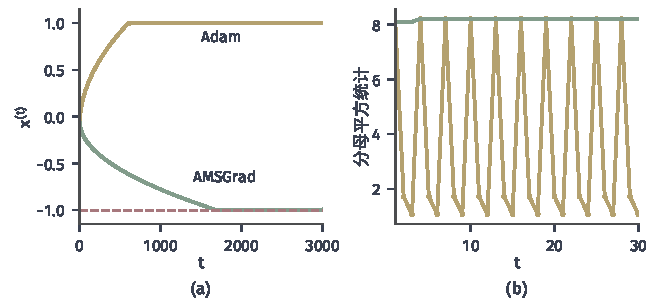
\includegraphics[width=112mm]{figures/05-optimization/05-stochastic-optimization/matplotlib/sgdb-amsgrad-counter/figure.pdf}
  \caption{周期线性目标上的Adam与AMSGrad，$C=3$，$\beta_1=0$，$\beta_2=0.1$，$\alpha^{(t)}=0.1/\sqrt t$，可行集$[-1,1]$。(a)迭代点，红色虚线是最优解$x=-1$。(b)分母中的平方统计：黄线是Adam随读数大幅涨落，绿线是AMSGrad保持最大值。}
  \label{fig:sgdb-amsgrad-counter}
\end{BookInlineFigure}

\paragraph{单调性是代数性质}
由更新规则，$\bar{\bm s}^{(t)}$逐坐标不减。若基步长$\alpha^{(t)}$不增，则每个坐标的有效缩放系数$\alpha^{(t)}/(\sqrt{\bar s_j^{(t)}}+\epsilon)$也不增。

这只是一个代数性质。它不说明目标值下降，也不说明算法收敛。AMSGrad的在线遗憾界需要凸性、有界可行域、有界读数，以及对$\beta_1^{(t)}$等参数的具体条件\scite{reddi2018amsgrad}；随机优化和非凸问题上的保证有各自的前提。不同问题上的结论不能互相代替。

\subsection{AdamW}
\label{sec:sgdb-adamw}

\paragraph{算法}
目标中常含平方惩罚$\frac\gamma2\lVert\bm{x}\rVert_2^2$。一种处理方式是把惩罚的梯度$\gamma\bm{x}$加到读数上，送进Adam的统计。另一种是\term{权重衰减}（weight decay）：历史统计只读取原目标的梯度，另外用更新前的参数单独收缩\scite{loshchilov2019adamw}。后一种方法称为AdamW，统计按式~\eqref{eq:sgdb-adam-stats}和式~\eqref{eq:sgdb-adam-correction}计算，参数更新改为
\begin{equation}
 \bm{x}^{(t+1)}=\bigl(1-\alpha^{(t)}\gamma\bigr)\bm{x}^{(t)}-\alpha^{(t)}\frac{\hat{\bm m}^{(t+1)}}{\sqrt{\hat{\bm s}^{(t+1)}}+\epsilon}.
 \label{eq:sgdb-adamw}
\end{equation}

收缩系数是$\alpha^{(t)}\gamma$，所以步长调度也带动收缩。对固定步长的随机梯度下降，两种做法相同：
\[
 \bm{x}-\alpha(\hat{\bm g}+\gamma\bm{x})=(1-\alpha\gamma)\bm{x}-\alpha\hat{\bm g}.
\]
但Adam的方向经过归一化，惩罚的梯度一旦进入统计，它的尺度也被归一化掉，两者不再相同。

\paragraph{同一标量首步比较}
取$x^{(0)}=1$，读数$\hat g^{(0)}=-0.1$，$\alpha=0.1$，$\gamma=0.5$，忽略$\epsilon$。第一轮的归一化方向等于读数的符号。AdamW用$\operatorname{sign}(-0.1)=-1$，按式~\eqref{eq:sgdb-adamw}，
\[
 x^{(1)}=(1-0.05)\cdot1+0.1=1.05.
\]

把惩罚梯度并入读数时，并入后的读数是$-0.1+0.5\cdot1=0.4$，符号变成$+1$，于是
\[
 x^{(1)}=1-0.1=0.9.
\]

两种做法的位移方向相反。图~\ref{fig:sgdb-adamw-step}显示了$\gamma$变化时的情况：AdamW的第一步关于$\gamma$连续变化；并入读数的做法在$\gamma=0.1$处突变，符号翻转后位移就不再随$\gamma$改变，惩罚的大小被归一化抹去了。

\begin{BookInlineFigure}
  \centering
  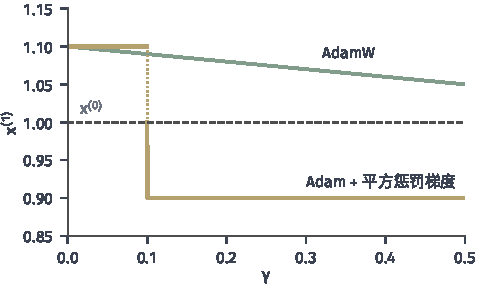
\includegraphics[width=82mm]{figures/05-optimization/05-stochastic-optimization/matplotlib/sgdb-adamw-step/figure.pdf}
  \caption{首步$x^{(1)}$关于惩罚系数$\gamma$的变化，$x^{(0)}=1$，$\hat g^{(0)}=-0.1$，$\alpha=0.1$。绿线是AdamW，黄线是把惩罚梯度并入读数后的Adam，虚线是起点。}
  \label{fig:sgdb-adamw-step}
\end{BookInlineFigure}

AdamW与平方惩罚并入读数的做法，优化的不是同一个迭代过程，它们停止的位置一般也不同。评价时要看实际定义的目标：返回点的目标值应写明是否包含惩罚项，收缩系数$\gamma$的含义也要随之说明。

\subsection{Adafactor统计压缩（补充）}
\label{sec:sgdb-adafactor}

\paragraph{用行列边际近似平方统计}
参数是矩阵$\bm{W}\in\mathbb{R}^{m\times d}$时，Adam的平方统计要存$md$个数。Adafactor只存平方统计的行和$\bm{r}\in\mathbb{R}^m$与列和$\bm{c}\in\mathbb{R}^d$，需要时重建近似的平方统计\scite{shazeer2018adafactor}。

设完整的平方统计是$\bm{V}$，$\bm{r}=\bm{V}\bm{1}_d$，$\bm{c}=\bm{V}^\top\bm{1}_m$。假定$\bm{V}$接近秩一，重建公式是
\begin{equation}
 \hat{\bm V}=\frac{\bm{r}\bm{c}^\top}{\bm{1}_m^\top\bm{r}} .
 \label{eq:sgdb-adafactor}
\end{equation}
分母是$\bm{V}$所有元素的和，这一归一化使重建保持行和与列和：$\hat{\bm V}\bm{1}_d=\bm{r}$，$\hat{\bm V}^\top\bm{1}_m=\bm{c}$。存储量从$md$降到$m+d$。

\paragraph{更新的次序}
一轮的次序是：先在读数的平方上加稳定项$\epsilon_1$，得到$\hat{\bm G}^{(t)}\odot\hat{\bm G}^{(t)}+\epsilon_1$，保证重建的分母为正；再分别用其行和与列和更新$\bm{r}$、$\bm{c}$的移动平均；然后由式~\eqref{eq:sgdb-adafactor}重建$\hat{\bm V}$；再求方向$\bm{Y}=\hat{\bm G}^{(t)}/\sqrt{\hat{\bm V}}$，把方向按均方根裁剪，最后乘以相对步长更新参数。相对步长与参数自身的均方根成正比，并有下界$\epsilon_2$。

这三件事分开算：统计压缩改变了尺度的来源，方向裁剪改变了方向的大小，相对步长改变了位移的量纲。评价改动带来的差别时，也要分别考虑。

\paragraph{保留与丢失的信息}
重建精确的条件很简单。若$\bm{V}$元素全为正，$\hat{\bm V}=\bm{V}$当且仅当$\bm{V}$秩为一，因为$\hat{\bm V}$按构造秩为一。例如
\[
 \bm{V}=\begin{bmatrix}1&2\\3&6\end{bmatrix}
\]
秩为一，行和是$(3,9)$，列和是$(4,8)$，总和是$12$，重建给出原矩阵。而
\[
 \bm{V}=\begin{bmatrix}4&1\\1&4\end{bmatrix}
\]
的行和、列和都是$(5,5)$，重建得到所有元素都是$2.5$的矩阵，对角线上的大值和非对角线的小值被抹平。

图~\ref{fig:sgdb-adafactor-recon}给出一个$6\times8$的例子。大尺度的行列结构被保留，逐元素的相对误差平均约为$0.13$，最大约为$0.70$。

\begin{BookInlineFigure}
  \centering
  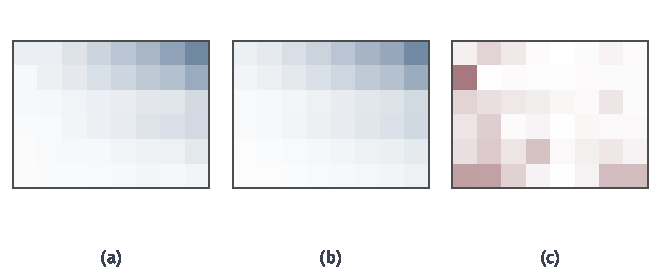
\includegraphics[width=112mm]{figures/05-optimization/05-stochastic-optimization/matplotlib/sgdb-adafactor-recon/figure.pdf}
  \caption{平方统计的行列压缩。(a)由$40$个随机读数算出的逐元素平方平均$\bm{V}$，形状$6\times8$。(b)按式~\eqref{eq:sgdb-adafactor}由$6$个行和与$8$个列和重建的$\hat{\bm V}$。(c)逐元素相对误差。颜色越深数值越大。}
  \label{fig:sgdb-adafactor-recon}
\end{BookInlineFigure}

压缩减少的只是统计的存储。参数、读数和方向仍是$md$个数；总计算量不会因此变成$O(m+d)$。低存储也不意味着收敛更快，近似的统计改变了方向，效果要回到目标上评价。

\subsection{Shampoo矩阵预条件（补充）}
\label{sec:sgdb-shampoo}

\paragraph{左右Gram统计}
逐坐标的尺度无法描述“某几行一起变化”这样的方向关系。Shampoo为矩阵参数维护左右两个Gram统计，分别刻画行空间和列空间方向的历史幅度\scite{gupta2018shampoo}。取$\epsilon>0$，$\bm{L}^{(0)}=\epsilon\bm{I}_m$，$\bm{R}^{(0)}=\epsilon\bm{I}_d$，读取矩阵读数$\hat{\bm G}^{(t)}$后先更新统计：
\begin{equation}
 \bm{L}^{(t+1)}=\bm{L}^{(t)}+\hat{\bm G}^{(t)}\hat{\bm G}^{(t)\top},\qquad
 \bm{R}^{(t+1)}=\bm{R}^{(t)}+\hat{\bm G}^{(t)\top}\hat{\bm G}^{(t)},
 \label{eq:sgdb-shampoo-stats}
\end{equation}
再用两侧的负四分之一次幂更新：
\begin{equation}
 \bm{W}^{(t+1)}=\bm{W}^{(t)}-\alpha\bigl(\bm{L}^{(t+1)}\bigr)^{-1/4}\hat{\bm G}^{(t)}\bigl(\bm{R}^{(t+1)}\bigr)^{-1/4}.
 \label{eq:sgdb-shampoo}
\end{equation}

$\epsilon$使两个统计正定，负四分之一次幂才有定义。按正交对角化计算：
\[
 \bm{L}=\bm{Q}\operatorname{diag}(\lambda_j)\bm{Q}^\top
 \quad\Longrightarrow\quad
 \bm{L}^{-1/4}=\bm{Q}\operatorname{diag}\bigl(\lambda_j^{-1/4}\bigr)\bm{Q}^\top .
\]
正交对角化可参考\BookChapterRef{chap:eigen-spectral-decomposition}{卷二第6章“谱分解”}。这两个矩阵是读数的累计，不是目标的Hessian。

\paragraph{单步：奇异值被拉平}
取$\epsilon\to0$，方阵可逆读数$\bm{G}=\bm{U}\bm{\Sigma}\bm{V}^\top$。则$\bm{G}\bm{G}^\top=\bm{U}\bm{\Sigma}^2\bm{U}^\top$，$\bm{G}^\top\bm{G}=\bm{V}\bm{\Sigma}^2\bm{V}^\top$，代入式~\eqref{eq:sgdb-shampoo}，
\[
 \bigl(\bm{G}\bm{G}^\top\bigr)^{-1/4}\bm{G}\bigl(\bm{G}^\top\bm{G}\bigr)^{-1/4}
 =\bm{U}\bm{\Sigma}^{-1/2}\bm{\Sigma}\bm{\Sigma}^{-1/2}\bm{V}^\top=\bm{U}\bm{V}^\top .
\]
一步的效果与Muon的理想极因子相同，所有奇异值都变成$1$。例如$\bm{G}=\operatorname{diag}(4,1/4)$时，两侧的变换都是$\operatorname{diag}(1/2,2)$，变换后得到$\bm{I}$，两个方向相差$16$倍的幅度被拉平。

累积多步之后不再这样简单。统计综合了历史上各方向的幅度，变换后的奇异值不等于$1$，并且随累积的读取逐渐减小，图~\ref{fig:sgdb-shampoo-flatten}(b)显示了这一点。这是累计式缩放的共同特点，与AdaGrad的有效系数逐渐减小相同。

\begin{BookInlineFigure}
  \centering
  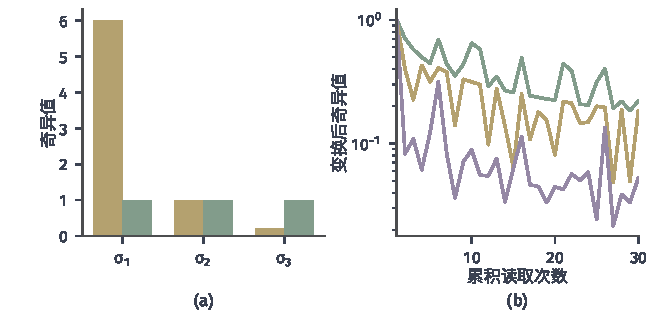
\includegraphics[width=112mm]{figures/05-optimization/05-stochastic-optimization/matplotlib/sgdb-shampoo-flatten/figure.pdf}
  \caption{Shampoo的奇异值变换，$\epsilon=10^{-6}$，$\bm{G}$是$3\times3$矩阵，奇异值为$6,1,0.2$。(a)单步：原始奇异值（黄）与式~\eqref{eq:sgdb-shampoo}变换后的奇异值（绿）。(b)累积读取时，变换后的三个奇异值随读取次数的变化，读数的各方向幅度随机变化。}
  \label{fig:sgdb-shampoo-flatten}
\end{BookInlineFigure}

\paragraph{计算成本}
Shampoo的额外成本比逐坐标方法高得多。统计的存储是$O(m^2+d^2)$；形成两个Gram矩阵需要$O(m^2d+md^2)$次运算；稠密谱分解求矩阵根一次约$O(m^3+d^3)$；两侧作用变换是$O(m^2d+md^2)$。

求根最贵，实际实现常隔若干步才重新计算根，中间继续使用旧因子。这样本轮使用的尺度来自若干步之前的统计，与式~\eqref{eq:sgdb-shampoo}“先更新后使用”不是同一个算法，记录时要写明刷新频率。比较方法时，统计存储、分解、旧因子的使用以及每步的乘法都要计入，不能只比较更新次数。
